\section{The Physics Impact of Alignment and Calibration}
\textcolor{red}{Importance of alignment and of rich pid selection (example run1).
To be included also effect of alignment on ip resolution.
To be added also something about the calorimeter calibration.}

The spatial alignment of a detector and the accurate calibration of its
subcomponents are essential to achieve the best physics
performance. The correct alignment of the VELO is needed to identify primary
vertices and secondary vertices from the decay of particles containing $b$ or
$c$ quarks while a misalignment of the tracking system would degrade the
momentum and mass resolution.  Figure~\ref{fig:Upsilon} shows how an improved
alignment greatly enhances the $\Upsilon$ mass resolution from $92$ MeV$/c^2$
with the first alignment to $49$ MeV$/c^2$ with the improved one.

\begin{figure}[h]
\begin{minipage}{0.5\columnwidth}
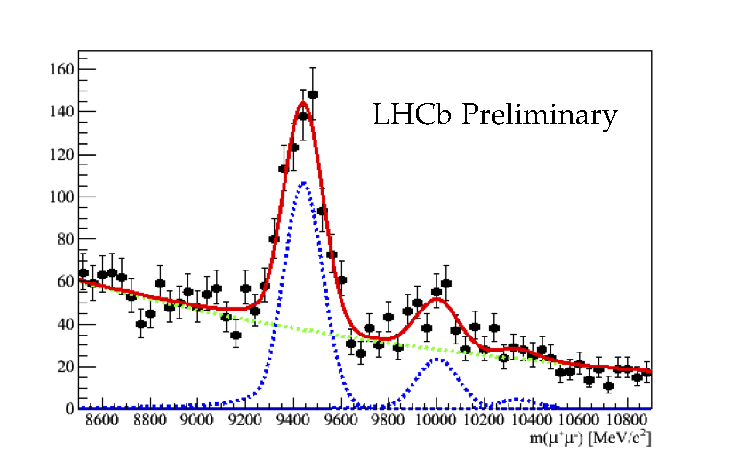
\includegraphics[width=\columnwidth]{../figures/Upsilon1}
\end{minipage}\hspace{2pc
}%
\begin{minipage}{0.5\columnwidth}
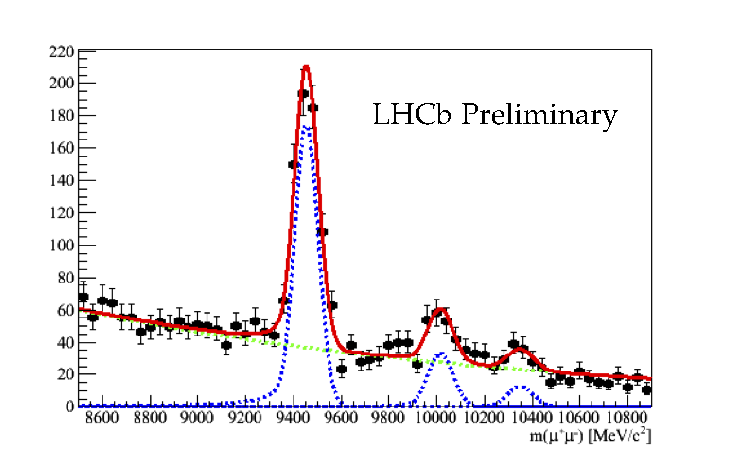
\includegraphics[width=\columnwidth]{../figures/Upsilon2}
\end{minipage} 
\caption{\label{fig:Upsilon} Invariant mass distribution for $\Upsilon \to \mu
  \mu$. The mass resolution is $92$
  MeV$/c^2$ with the first alignment (left) and is enhanced to $49$
  MeV$/c^2$ with an improved alignment (right).}
\end{figure}

An exclusive selection using hadron identification criteria relies on the
complete calibration of the ring-imaging Cherenkov
detectors. Figure~\ref{fig:PID} shows the effect in the $B^0\to h^+ h^-$ mass
spectrum of hadron identification criteria: the ratio between the signal,
$B^0\to\pi^+\pi^-$, and the combinatorial background increases by approximately
a factor two and the ratio between the signal and the favoured $B^0\to K \pi$,
increases by a factor 35.
\begin{figure}[h]
\begin{minipage}{0.5\columnwidth}
\includegraphics[width=\columnwidth]{../figures/PID1}
\end{minipage}\hspace{2pc}%
\begin{minipage}{0.5\columnwidth}
\includegraphics[width=\columnwidth]{../figures/PID2}
\end{minipage} 
\caption{\label{fig:PID} Invariant mass distribution for $B^0\to h^+ h^-$ decays~\cite{LHCb-PAPER-2012-002} in
  the LHCb data before the use of the RICH information (left), and after
  applying RICH particle identification (right). The signal under study is the
  decay $B^0\to\pi^+\pi^-$, represented by the turquoise dotted line. The
  contributions from different $b$-hadron decay modes ($B^0\to K\pi$ red dashed-dotted
  line, $B^0\to 3$-bodies orange dashed-dashed line, $B_s\to
    KK$ yellow line, $B_s\to K\pi$
  brown line, $\Lambda_b\to p K$ purple line, $\Lambda_b\to p \pi$ green line), are eliminated by
  positive identification of pions, kaons and protons. Only the signal and
  two background contributions remain visible after applying hadron
  identification requirements. The
  grey solid line is the combinatorial background.}
\end{figure}

\begin{figure}[h]
\begin{minipage}{0.5\columnwidth}
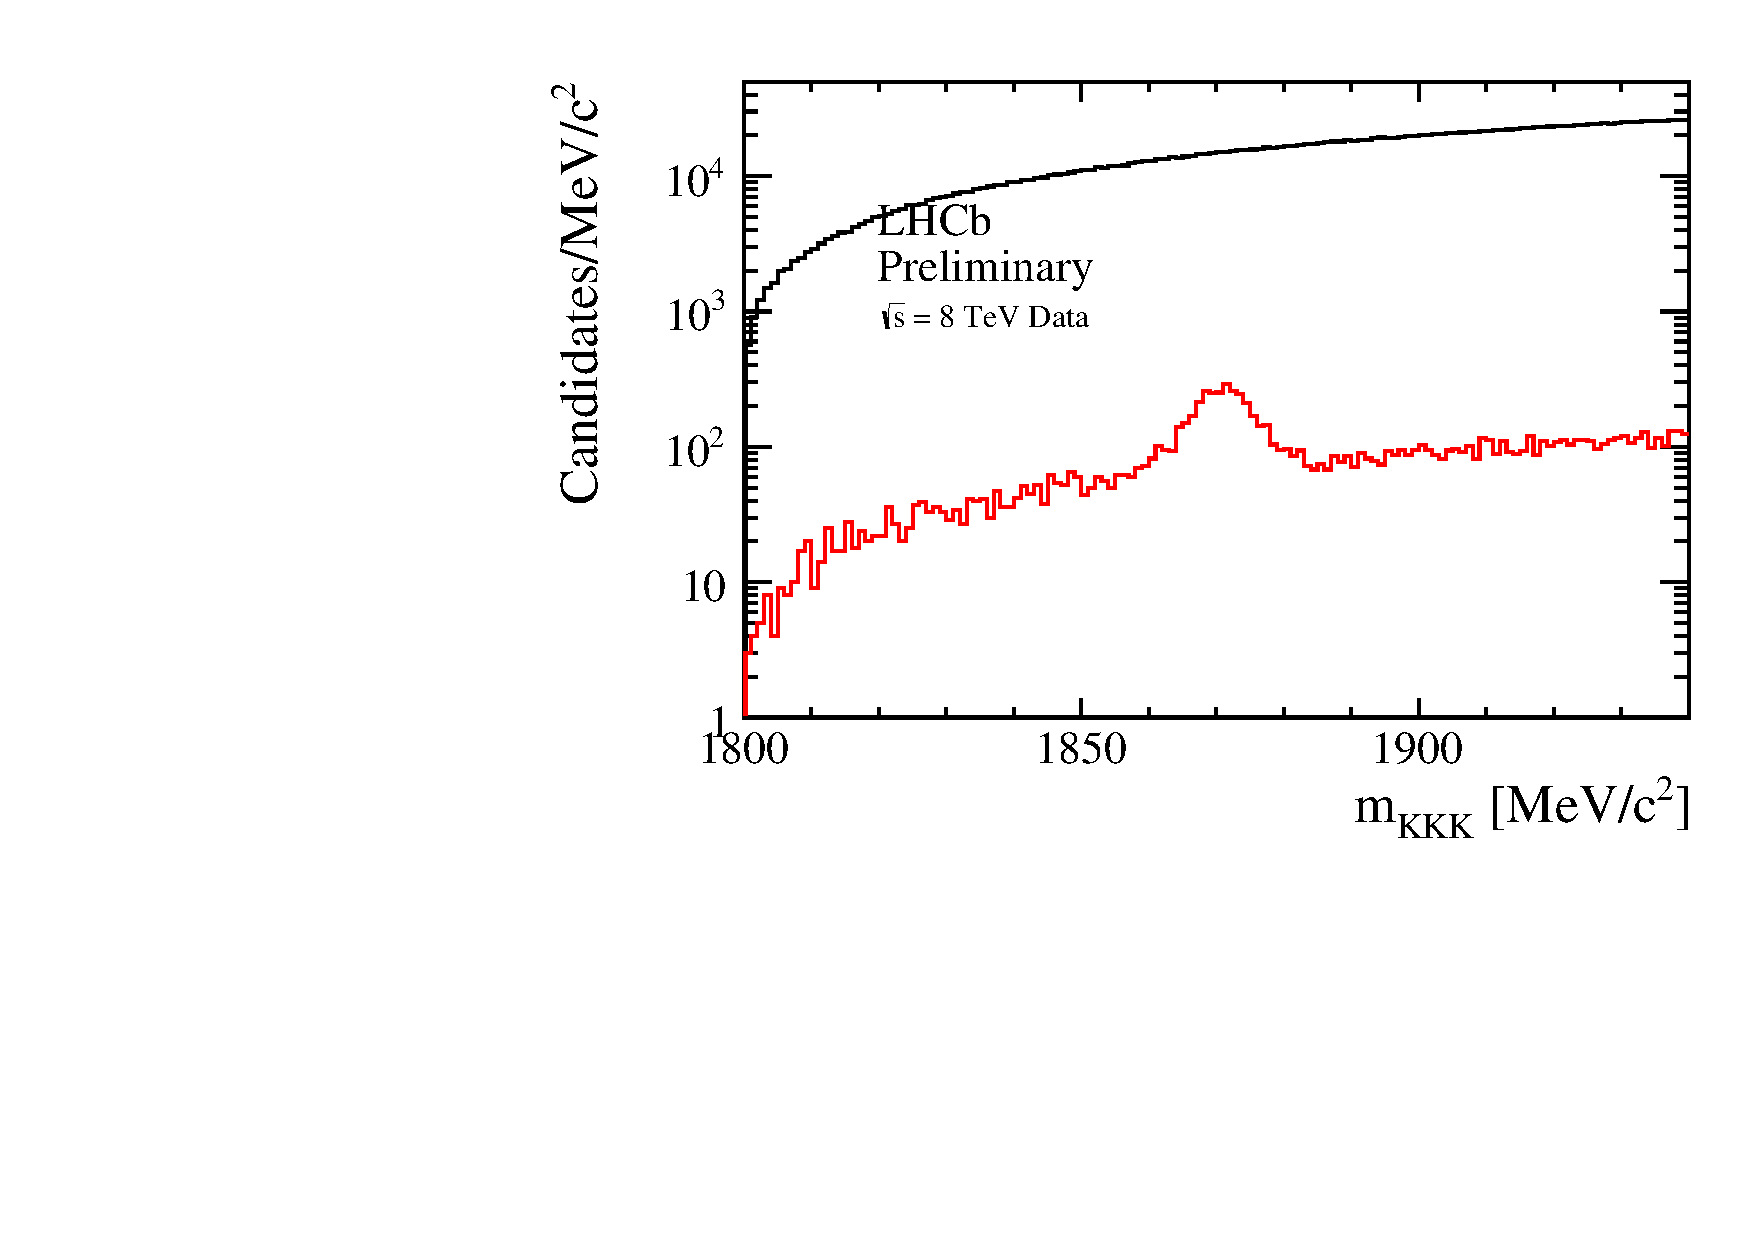
\includegraphics[width=\columnwidth]{../figures/kkk_PIDK_trigger_log}
\end{minipage}\hspace{2pc}%
\begin{minipage}{0.5\columnwidth}
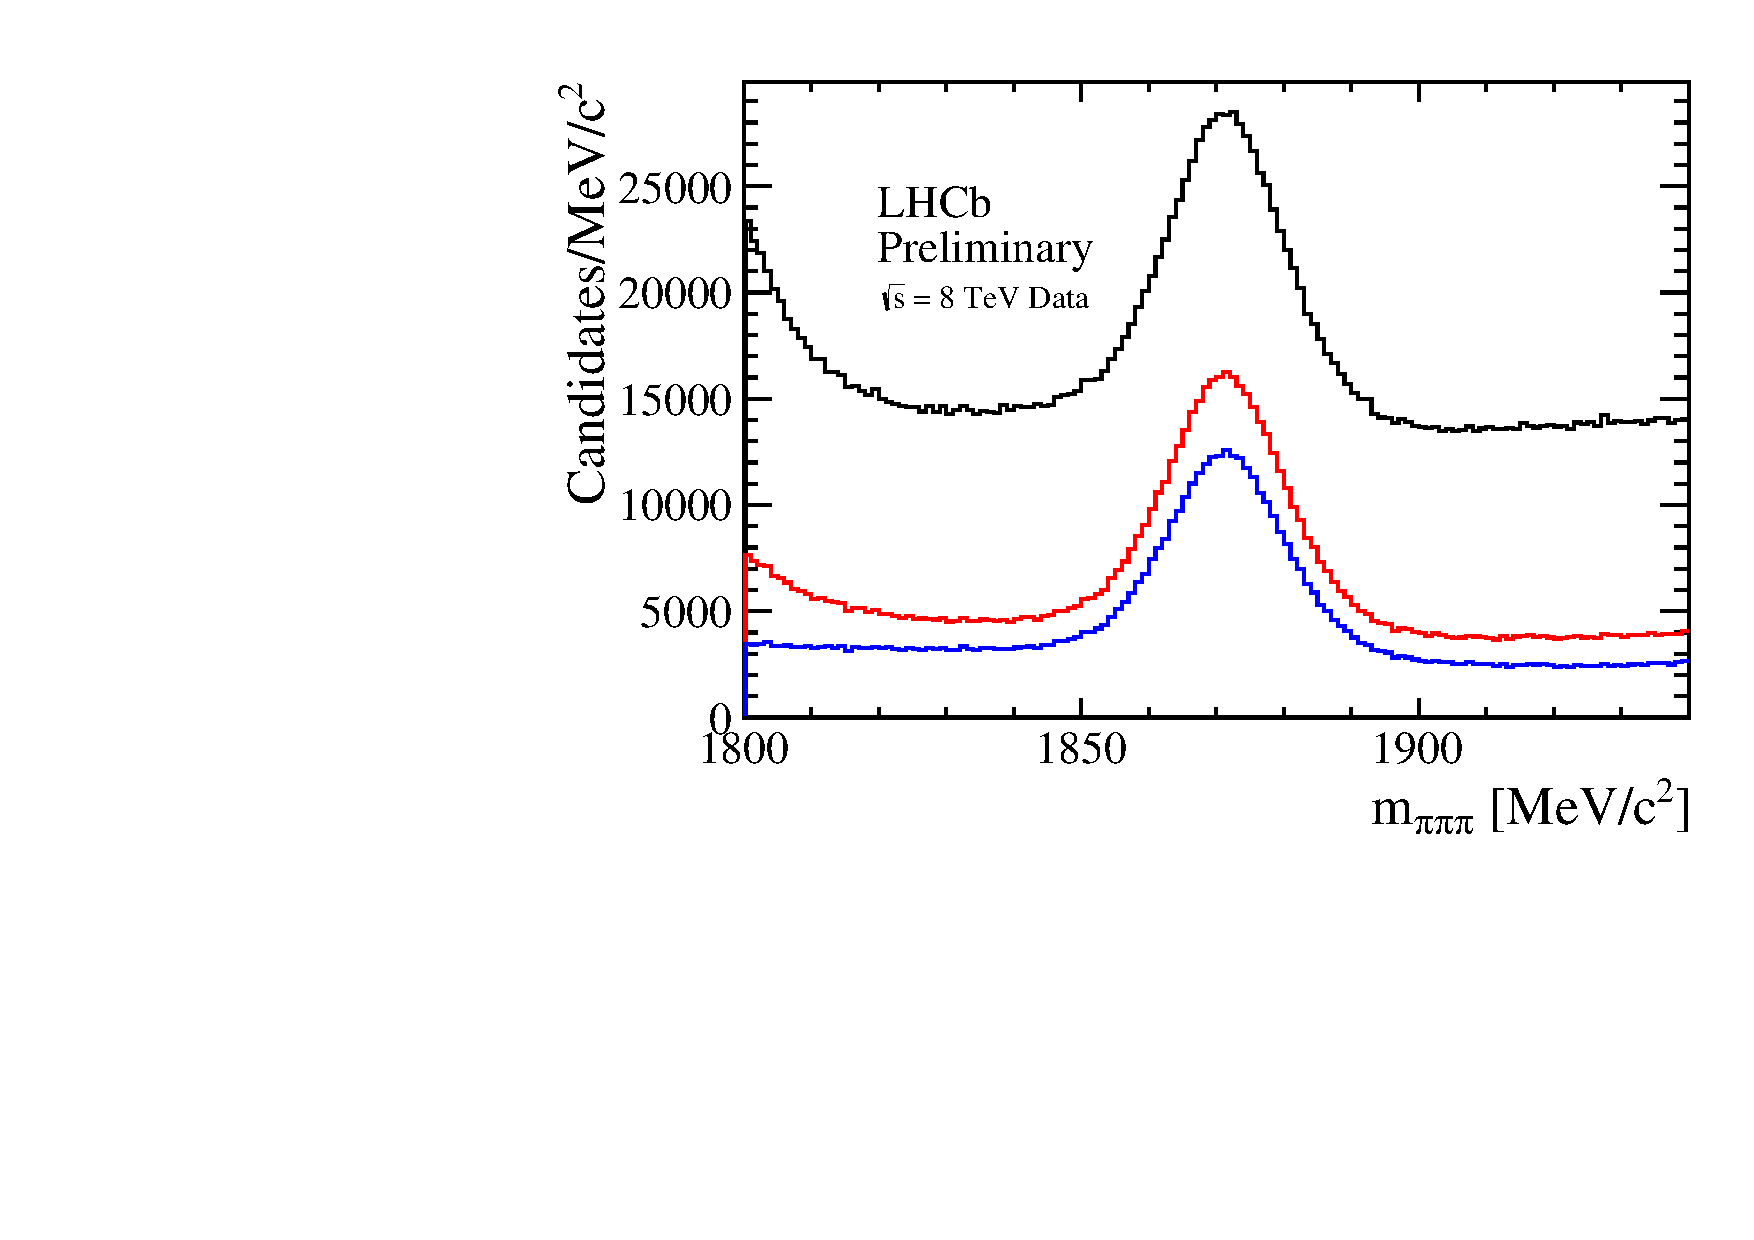
\includegraphics[width=\columnwidth]{../figures/ppp_PIDK_trigger}
\end{minipage} 
\caption{\label{fig:CharmPID} 3 body decay distribution for D0 to  kkkk (left) and pipipi (right). To be written  }
\end{figure}

Is it thus clear that using a real-time alignment and calibration during the
trigger selection allows a higher signal purity and a more effective selection
on the channels interesting to pursue LHCb's physics program without increasing
the overall trigger rate. This, however, requires us
to align more than 1700 detector components and compute almost 2000
calibration constants in real-time. It is therefore important to understand the frequency
with which the relevant constants are expected to vary.

The VELO is made of two halves that during the data taking are at approximately
8 mm away from the nominal beam position. For the safety of the detector during
the beam injection at the beginning of a fill the halves are retracted by 29 mm;
when stable beam is declared the VELO is closed around the beam.
The VELO halves are moved using stepper motors and their position is read from
resolvers mounted on the motor axes with an accuracy better than 10 $\mu$m.  An
automated closing procedure positions the VELO halves around the beams using the
response of the hardware and the measured positions of the beams.  By
considering the two independent beam profiles compiled by each half, the VELO is
observed to close symmetrically around the beams to an accuracy of better than 4
$\mu$m.  As the VELO is closed for each fill, its alignment may change with the
same frequency.

Figure \ref{fig:alignStability} shows for a subsample of the Run~I dataset the
variation of the misalignment between the two halves in the horizontal direction
perpendicular to the beam. It can be estimated by taking the difference of the
positions of the primary vertices reconstructed separately with tracks in only
one half of the VELO. In a perfectly aligned detector the mean of this
difference should be zero. The average variation in Run~I is $\sim 4\,\mu$m
while the maximum variation is $O(10\,\mu$m$)$, which is more than the
$O(2\,\mu$m$)$ precision of the track based software alignment procedure
\cite{LHCb-DP-2014-001}.

\begin{figure}[h]
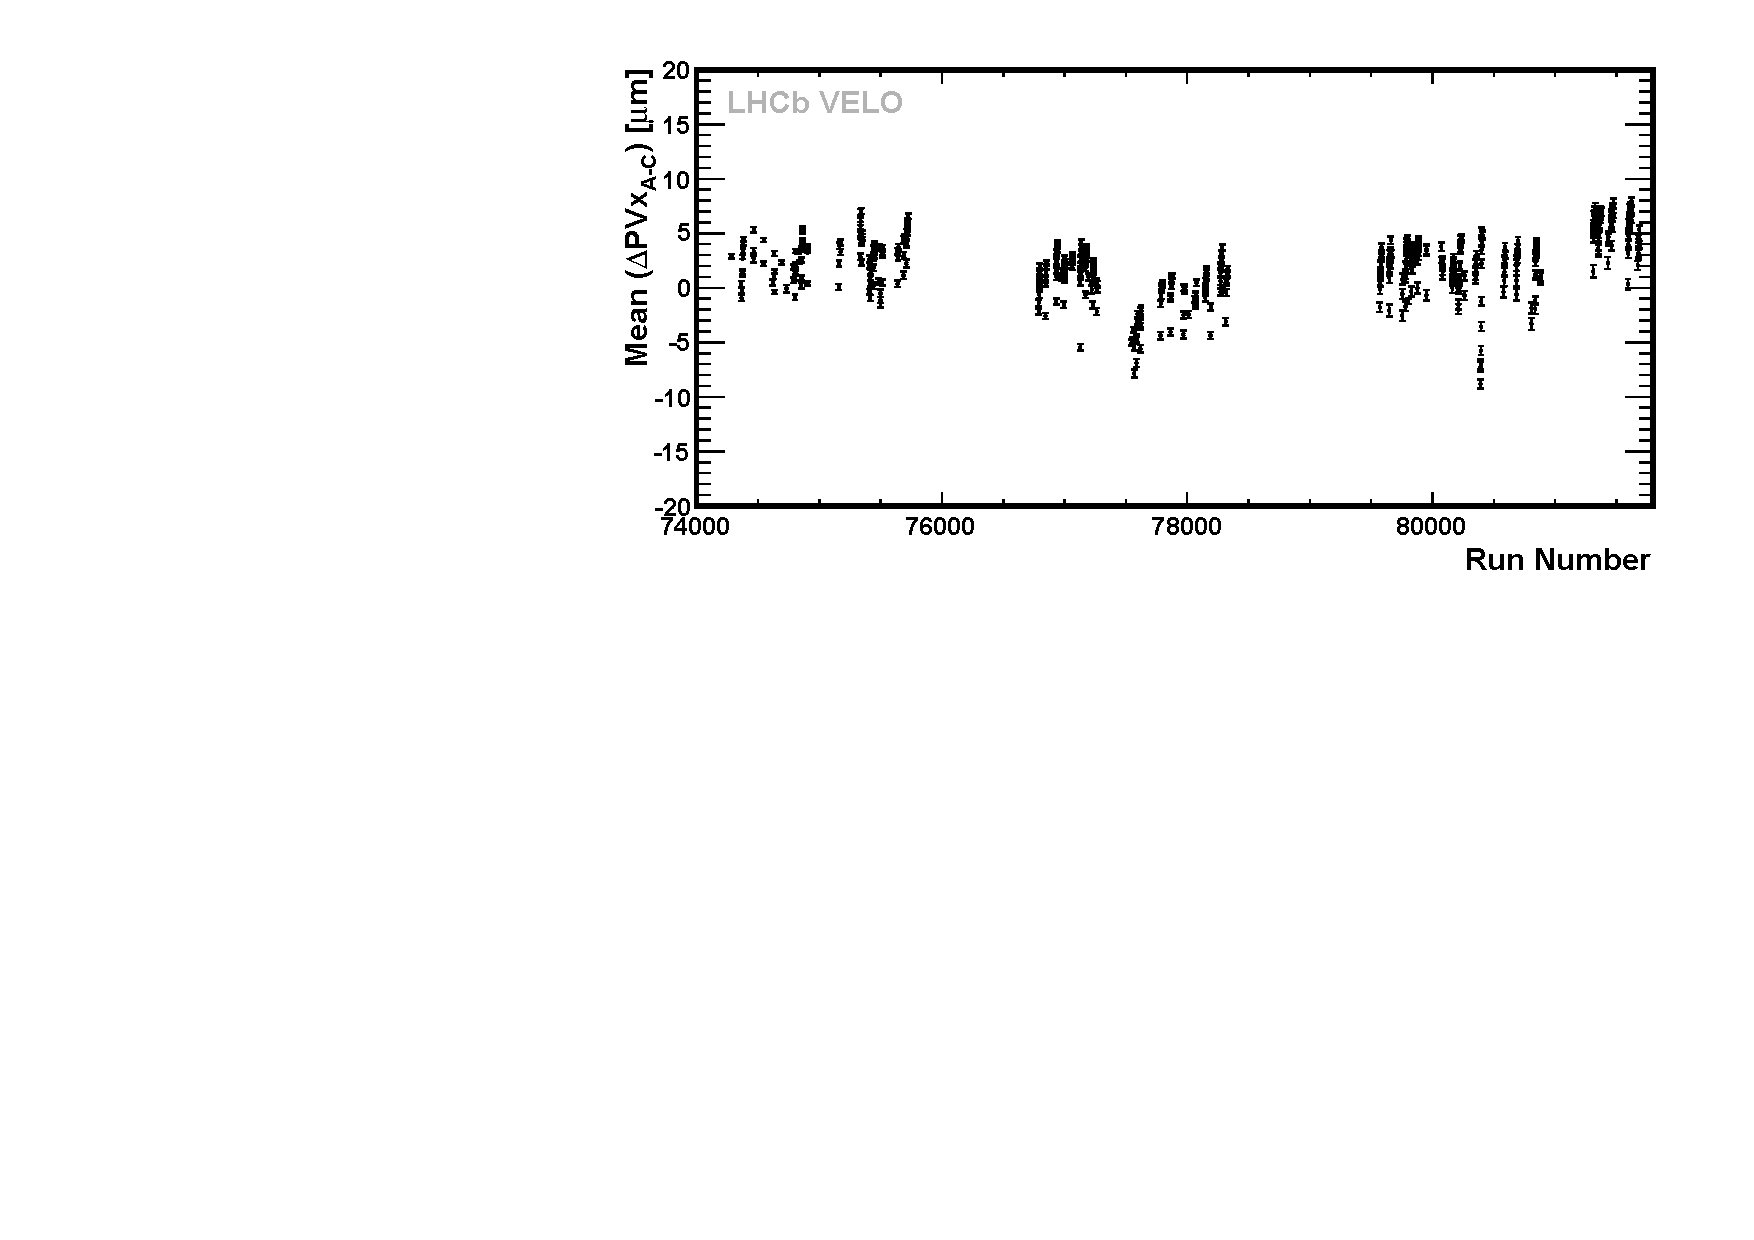
\includegraphics[width=20pc]{../figures/alignStability}\hspace{2pc}%
\begin{minipage}[b]{14pc}\caption{\label{fig:alignStability}
    Misalignment 
    between the two VELO halves along the main movement direction
    for the different runs, evaluated by fitting the primary
    vertices separately with tracks in each half of the VELO. 
The run numbers shown here span the period of the last four months of operations in 2010.}
\end{minipage}
\end{figure}

For the other components of the tracking system, in addition to the variation
due to hardware intervention, some variation over time was observed, partially
correlated to the magnet polarity which is reversed periodically. During Run~I a
new tracking alignment has been evaluated after each magnet polarity switch or
technical stop.  This strategy allowed to have a momentum scale and resolution
stable with time as shown in Figure \ref{fig:trackerStability}.

\begin{figure}[h]
\begin{minipage}{0.5\columnwidth}
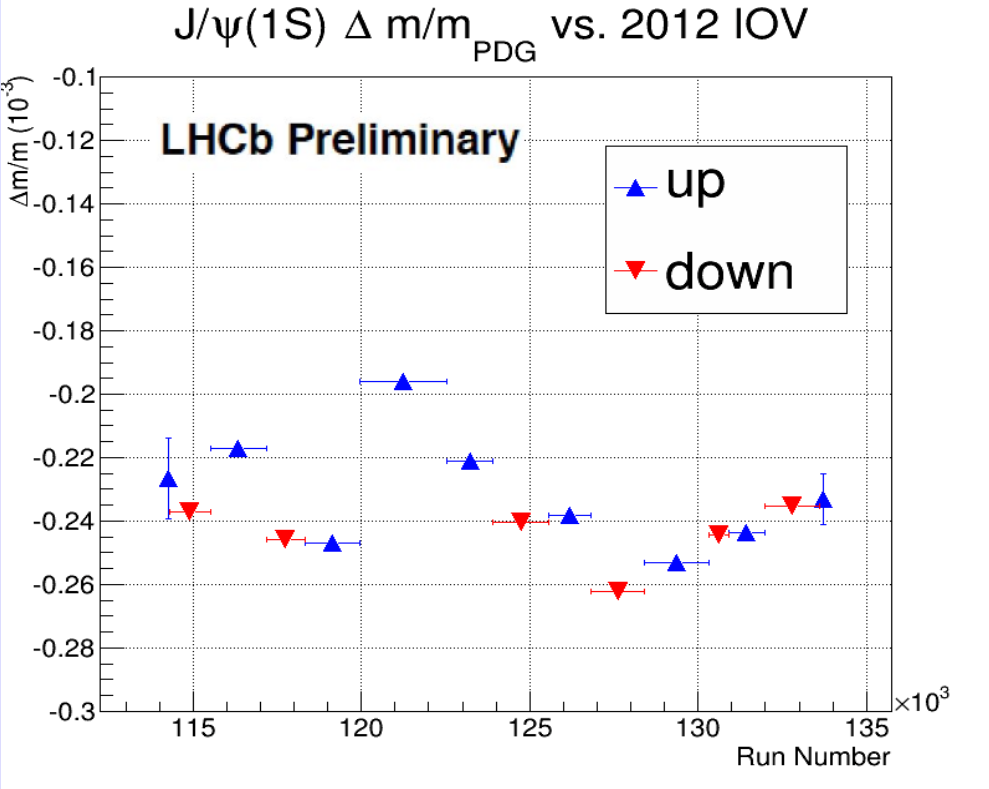
\includegraphics[width=\columnwidth]{../figures/JPsi1.png}
\end{minipage}\hspace{2pc}%
\begin{minipage}{0.5\columnwidth}
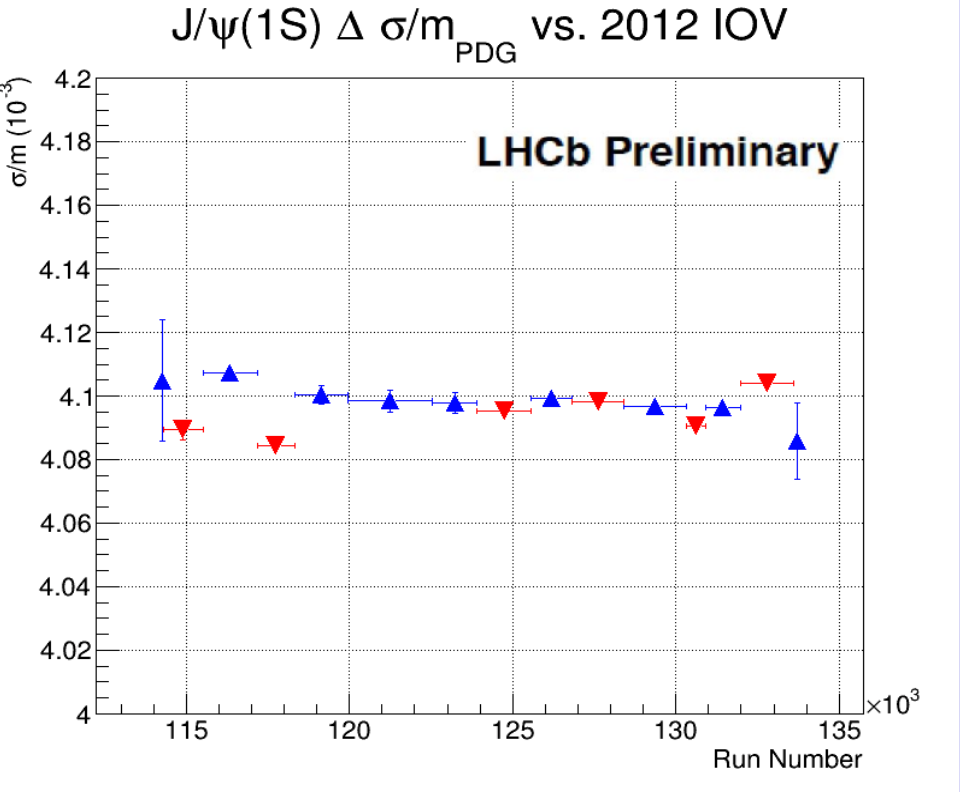
\includegraphics[width=\columnwidth]{../figures/JPsi2.png}
\end{minipage} 
\caption{\label{fig:trackerStability} Time evolution of  the relative variation of the difference
  between the measured mass of the $J/\Psi$(1S) and the nominal one from
  \cite{PDG} (left) and relative variation of the mass resolution at the
  $J/\Psi$(1S) mass (right). Each point corresponds to data taken with a
  different tracking alignment; the blue up-triangles and red down-triangles correspond to opposite magnet polarities.}
\end{figure}

Finally, in the case of the gaseous RICH detectors, the variations of temperature
and pressure in the experimental cavern mean that the refractive index of the gas
changes continuously. In order to achieve the best particle identification performance, it 
is necessary to compute these constants for each run. On the other hand, the alignment
of the RICH mirrors is seen to vary only infrequently, and in general only needs to be updated
after an extended shutdown of the detector. \textbf{DO WE HAVE SOME JUSTIFICATION?}

\textbf{SAY SOMETHING ABOUT THE EXPECTED VARIATION OF THE CALO HERE?}
